

%%%%%%%%%%%%%%%%%%%%%%%%%%%%%%%%%%%%%%%%%%%%%%%%%%%%%%%%%%%%%%%%%%%%%%%%%%%%%%%%%%
%%%%%%%%%%%%%%%%%%%%%%%%%%%%%%%%%%%%%%%%%%%%%%%%%%%%%%%%%%%%%%%%%%%%%%%%%%%%%%%%%%
\begin{frame}
  \begin{small}
              
  \begin{columns}
  \column{0.9\textwidth}
    \hhref{https://wir2022.wid.world/download}{World Inequality Report 2022}
    \begin{itemize}\setlength\itemsep{1.0ex}\footnotesize
      \item[o] Beautifully presented data on regional and societal inequalities in income, wealth, and carbon emissions
    \end{itemize}
  \end{columns}

  \end{small}
  \end{frame}

%%%%%%%%%%%%%%%%%%%%%%%%%%%%%%%%%%%%%%%%%%%%%%%%%%%%%%%%%%%%%%%%%%%%%%%%%%%%%%%%%%
\begin{frame}
  \frametitle{\centerline{ \hhref{https://wir2022.wid.world/download/}{World Inequality Report:} Total CO$_2$ emissions per region}}
  \begin{scriptsize}

    \begin{columns}
      \column{1.0\textwidth}
      \begin{itemize}\setlength\itemsep{1.3ex}        
        \item[o] {\cb Left:} This graph shows the breakdown of the global CO$_2$ emissions by major economic regions as a function of time. Total global CO$_2$ emissions in 2019 were 50 billion tonnes. After 1990, emissions include carbon and other greenhouse gases embedded in imports/exports of goods and services from/to other regions. {\it Close to half (46\%) of historical CO$_2$ emissions were released after 1990.}

        \item[o] {\cb Right:} The graph shows historical emissions by region (left bar) and the remaining global carbon budget (centre and right bars) to have 83\% chances to stay under 1.5°C and 2°C, according to IPCC Assessment Report 6 (2021). Regional emissions are net of carbon embedded in imports of goods and services from other regions.
    \end{itemize}

    \end{columns}

    \vspace{0.4cm}
    \begin{columns}
      \column{0.6\textwidth}
      \begin{center}
          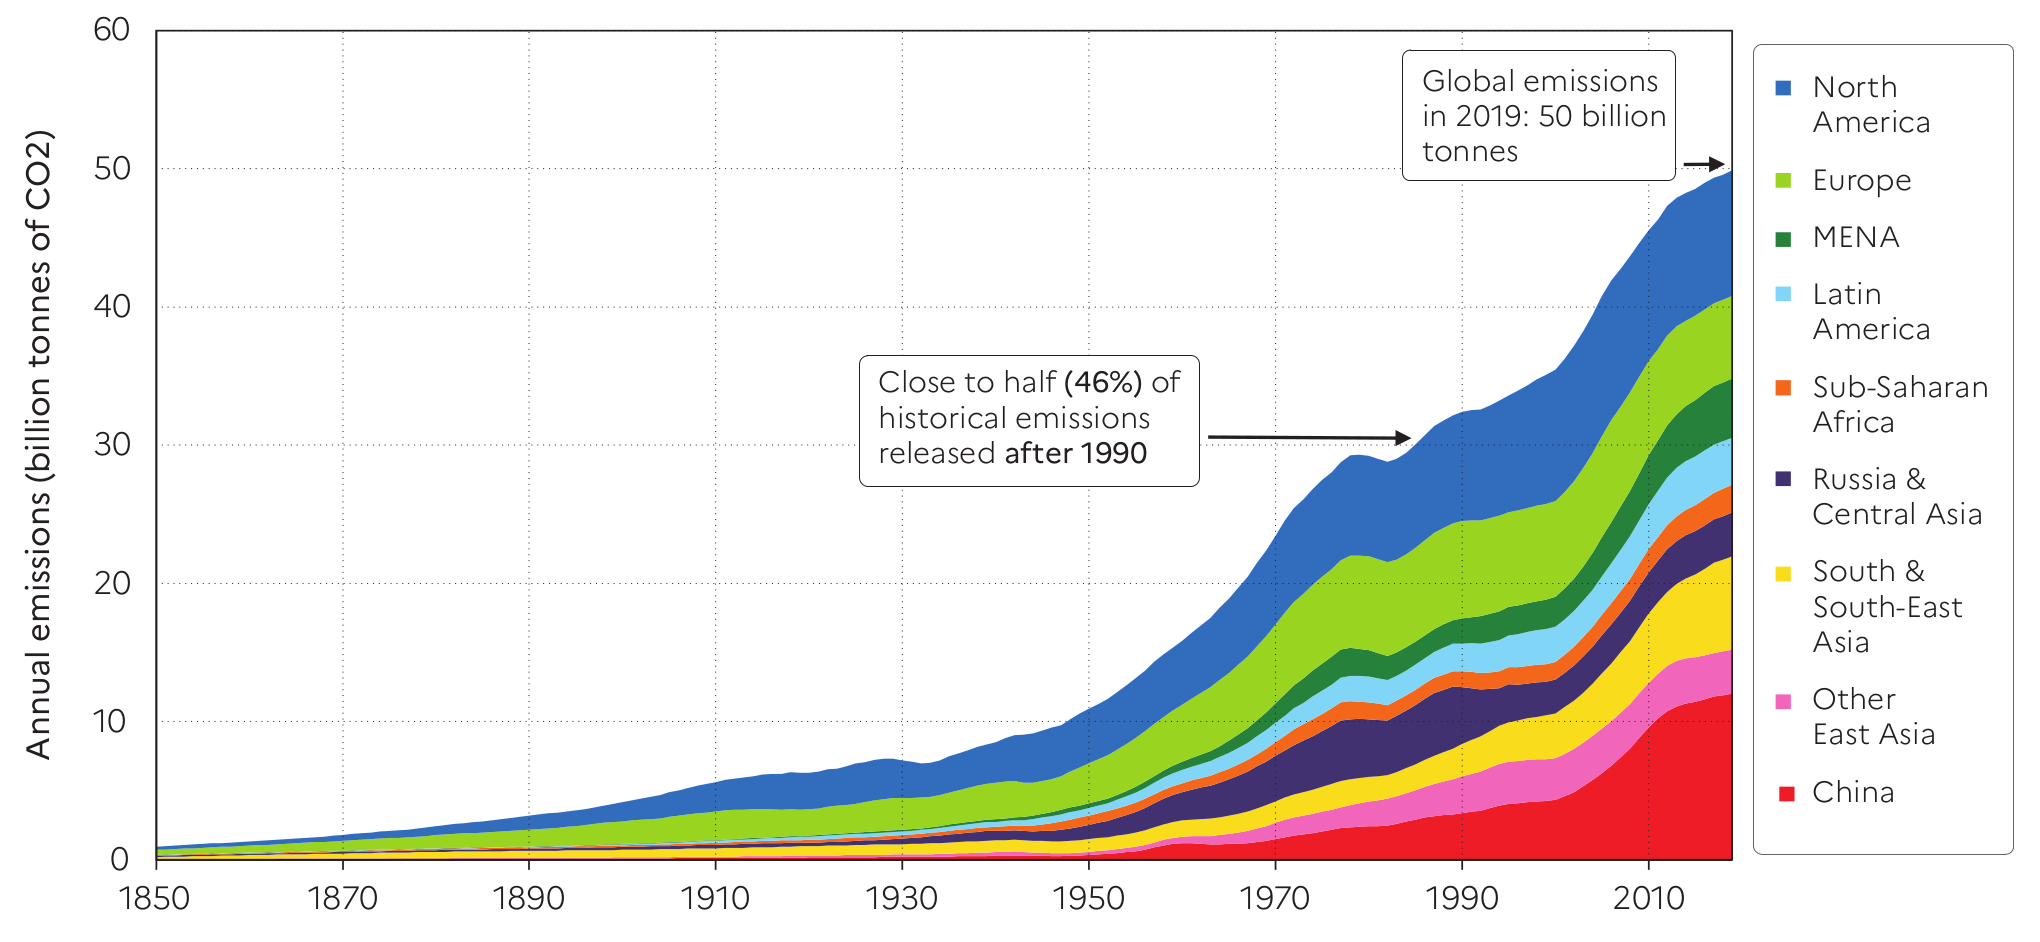
\includegraphics[width=1.0\textwidth]{plots/WIR_co2_per_region_vs_time}
      \end{center}

      \column{0.5\textwidth}
      \begin{center}
        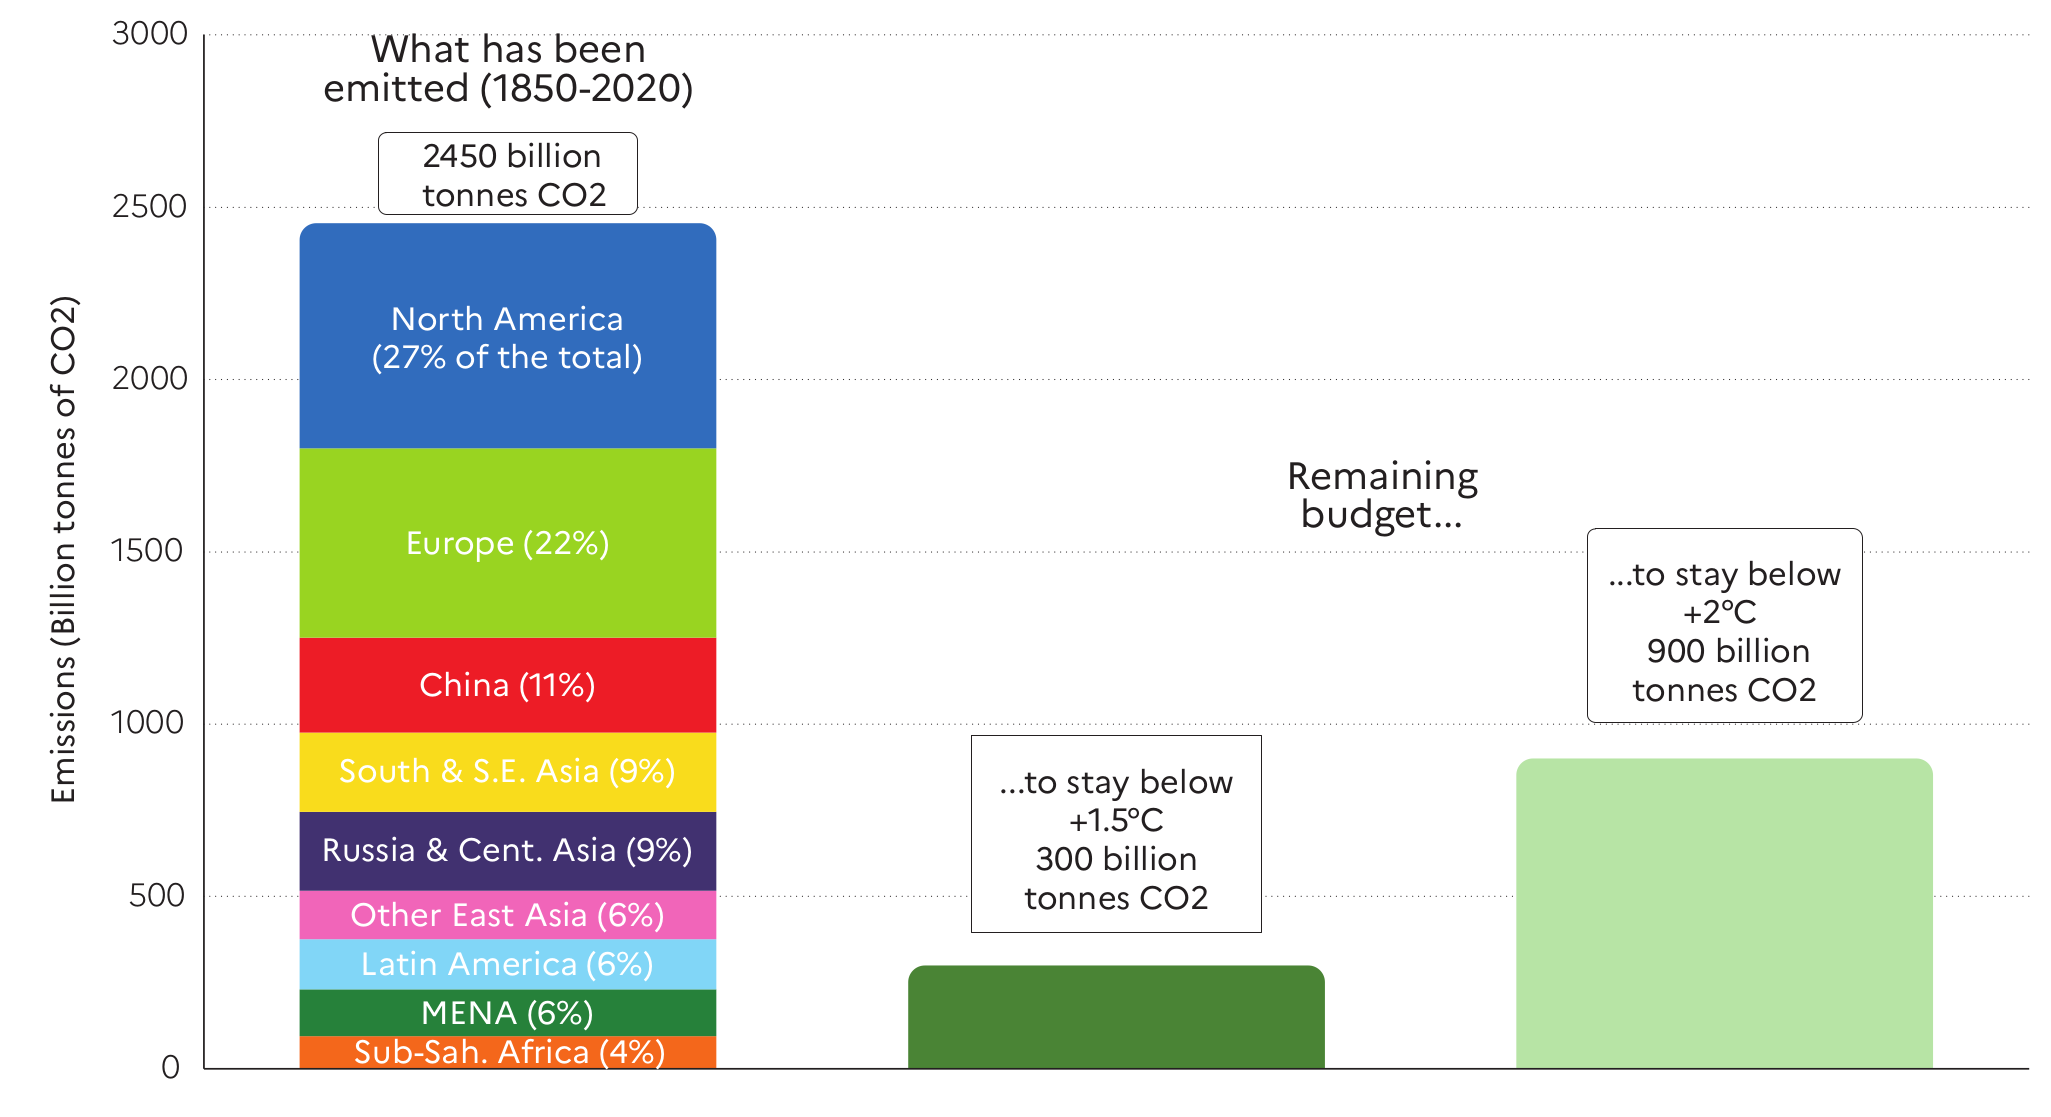
\includegraphics[width=1.0\textwidth]{plots/WIR_budget_emitted_and_allowed}
      \end{center}      
    \end{columns}

  \end{scriptsize}
  \end{frame}  

%%%%%%%%%%%%%%%%%%%%%%%%%%%%%%%%%%%%%%%%%%%%%%%%%%%%%%%%%%%%%%%%%%%%%%%%%%%%%%%%%%
\begin{frame}
  \frametitle{\centerline{ \hhref{https://wir2022.wid.world/download/}{World Inequality Report:} Average per capita CO$_2$ emissions in 2019}}
  \begin{scriptsize}

    \begin{columns}
      \column{1.0\textwidth}
      \begin{itemize}\setlength\itemsep{1.3ex}        
        \item[o] {\cb Left:} CO2 emissions in tonnes per capita, per year for different regions. The world average is 6.6 tons per capita. This needs to go down to 3.4 tons in order to limit global warming to 2 degrees above the pre-industrial level.

        \item[o] {\cb Right:} {\it The top 10\% of emitters are responsible for close to 50\% of all emissions, while the bottom 50\% produce 12\% of the total.}

        \item[o] Personal carbon footprints include emissions from domestic consumption, public and private investments as well as imports and exports of carbon embedded in goods and services traded with the rest of the world.
    \end{itemize}
    \end{columns}

    \vspace{0.4cm}
    \begin{columns}      
      \column{0.4\textwidth}
      \begin{center}
          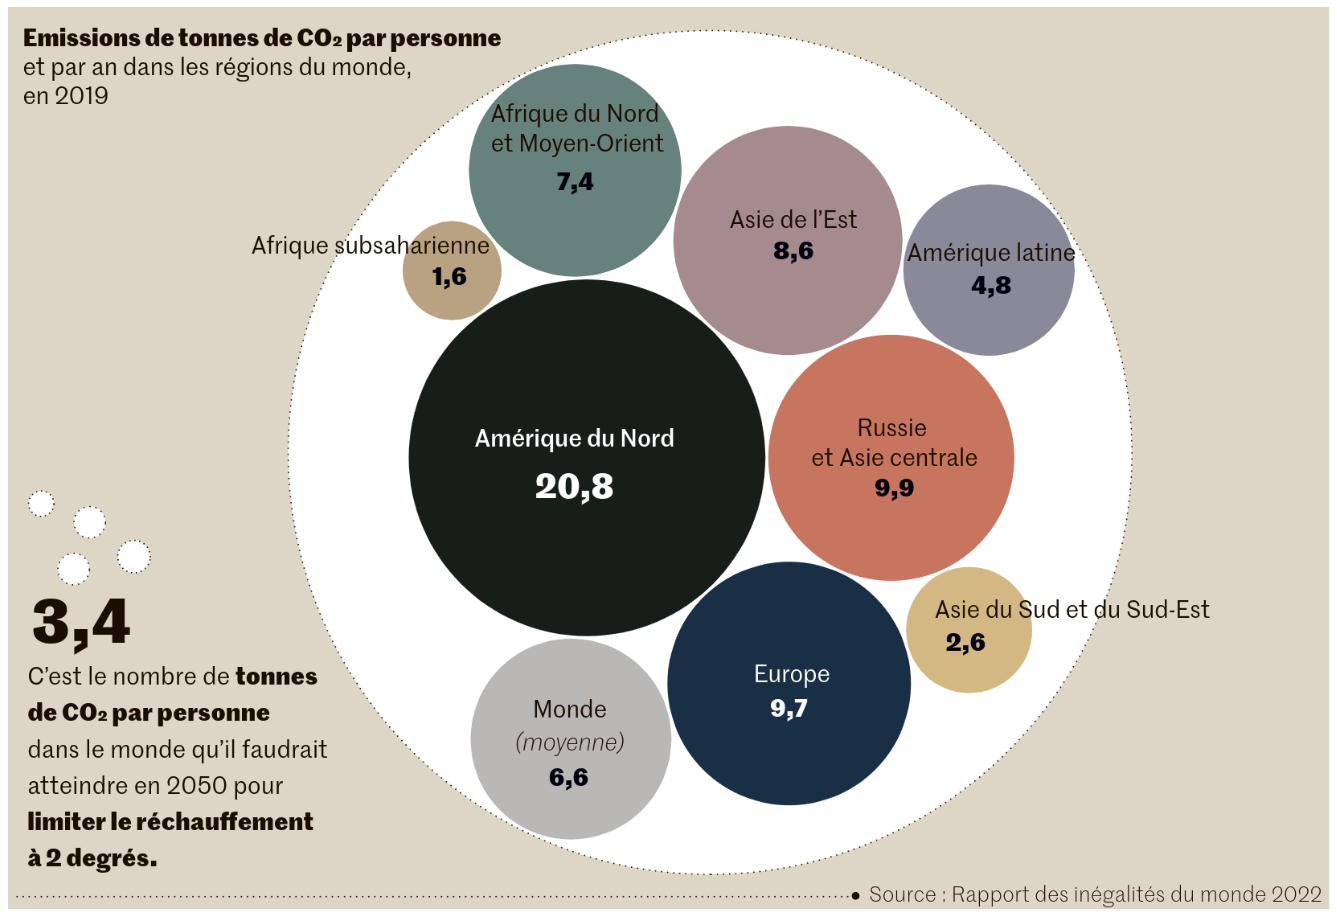
\includegraphics[width=1.0\textwidth]{plots/co2.png}
      \end{center}  

      \column{0.6\textwidth}
      \begin{center}
          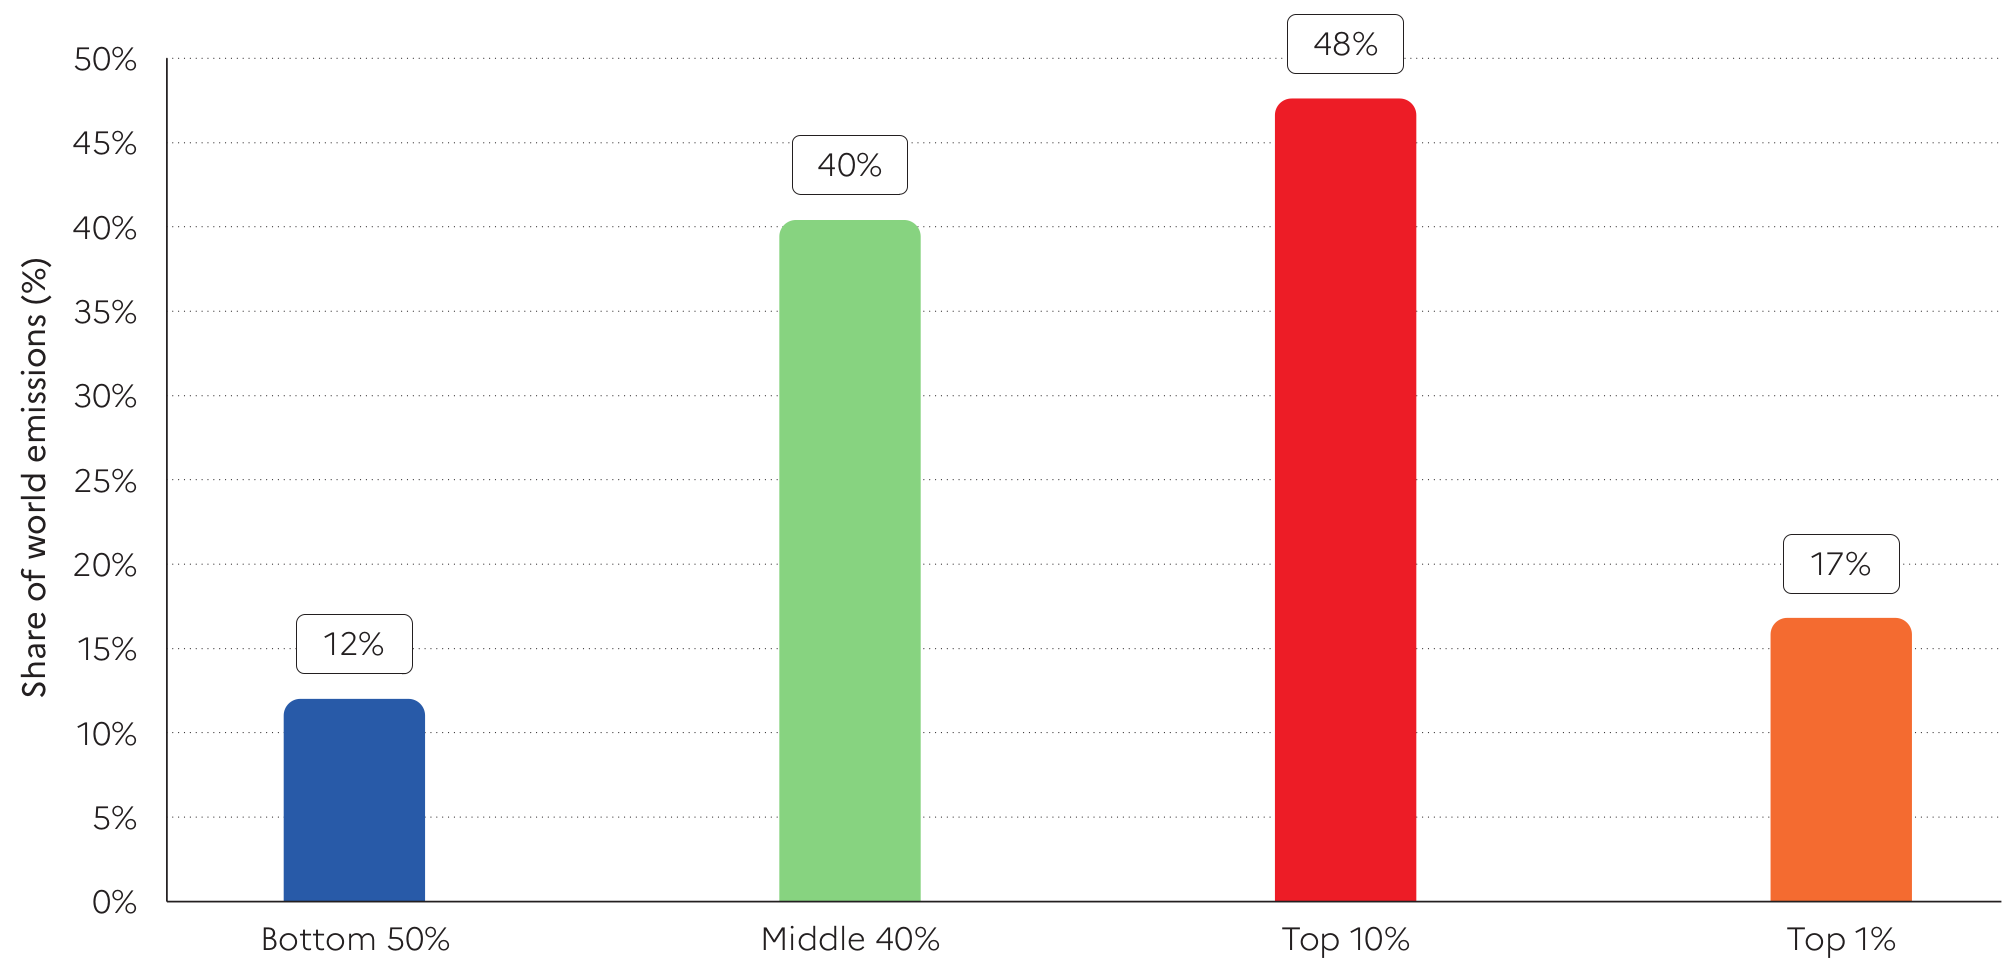
\includegraphics[width=1.0\textwidth]{plots/WIR_budget.png}
      \end{center}
    \end{columns}

  \end{scriptsize}
  \end{frame}  

%%%%%%%%%%%%%%%%%%%%%%%%%%%%%%%%%%%%%%%%%%%%%%%%%%%%%%%%%%%%%%%%%%%%%%%%%%%%%%%%%%
\begin{frame}
  \frametitle{\centerline{ \hhref{https://wir2022.wid.world/download/}{World Inequality Report:} Breakdown of per capita CO$_2$ emissions}}
  \begin{scriptsize}

    \begin{columns}
      \column{1.0\textwidth}
      \begin{itemize}\setlength\itemsep{1.3ex}        
        \item[o] CO$_2$ emissions of bottom 50\% of emitters per capita per year: 5 tonnes in Europe, 13 tonnes in East Asia, 10 tonnes in North America.

        \item[o] CO$_2$ emissions of top 10\% of emitters per capita per year: 29 tonnes in Europe, 39 tonnes in East Asia, 73 tonnes in North America.

        \item[o] Poorest half of the population in rich countries is already at (or near) the 2030 climate per-capita targets set by rich countries. This is not the case for the top half of the population. Large inequalities in emissions suggest that climate policies should target wealthy polluters more. So far, climate policies such as carbon taxes have often disproportionately impacted low and middle-income groups, while leaving the consumption habits of wealthiest groups unchanged.
    \end{itemize}
    \end{columns}

    \begin{columns}
      \column{0.5\textwidth}
      \begin{center}
          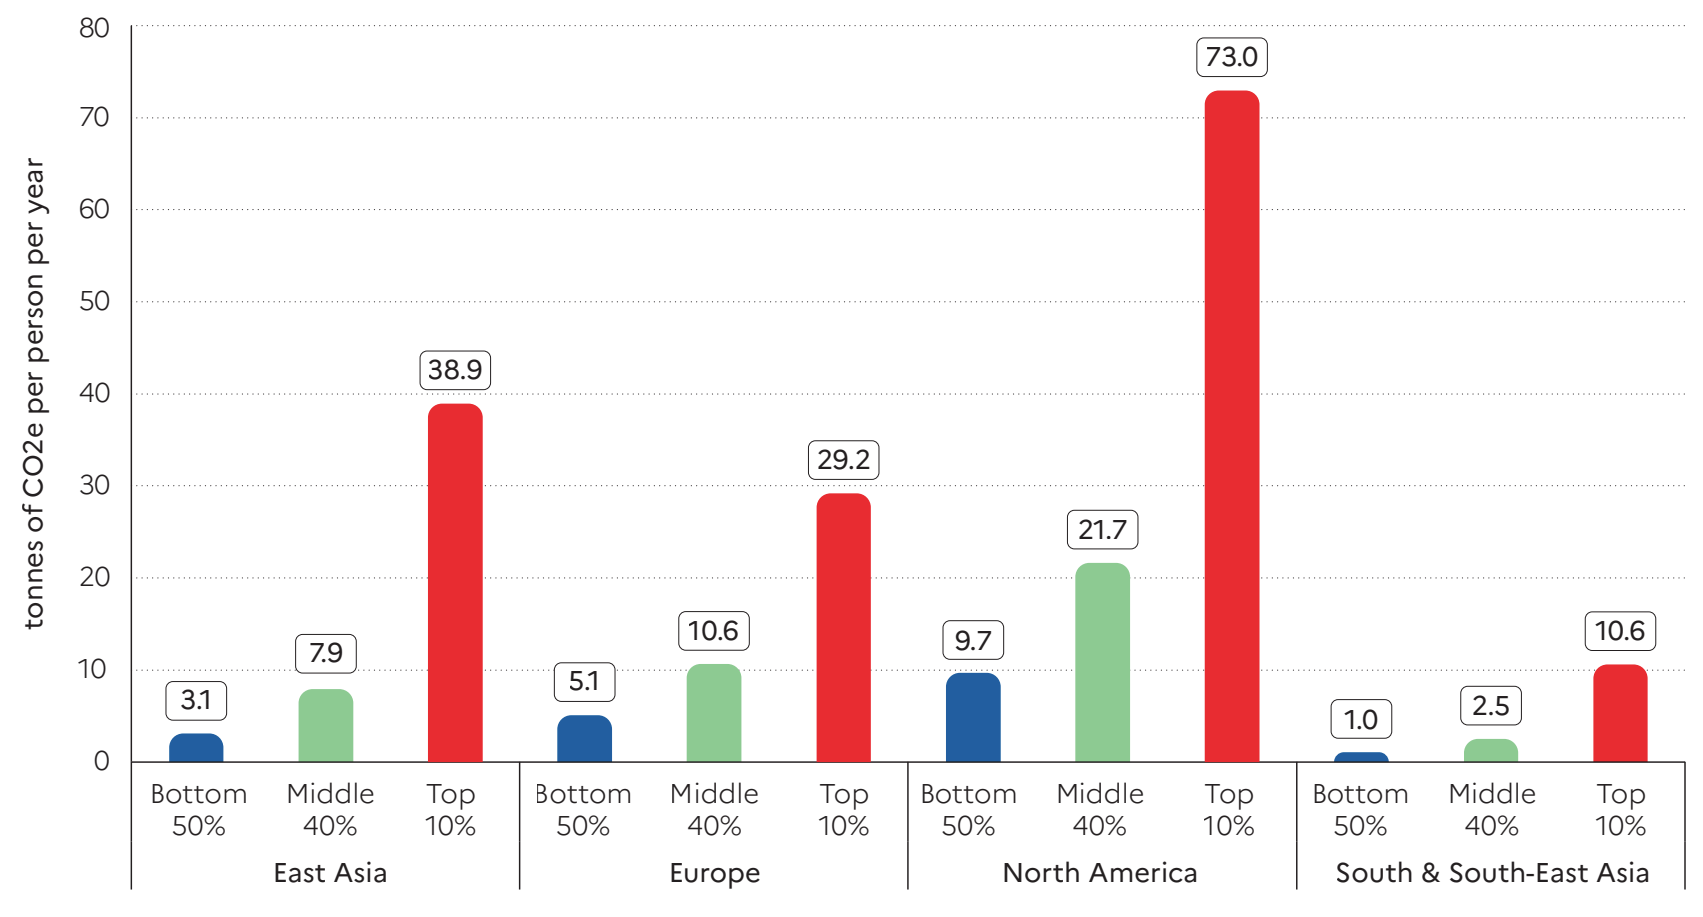
\includegraphics[width=1.0\textwidth]{plots/WIR_carbon_per_capita_west.png}
      \end{center}

      \column{0.5\textwidth}
      \begin{center}
        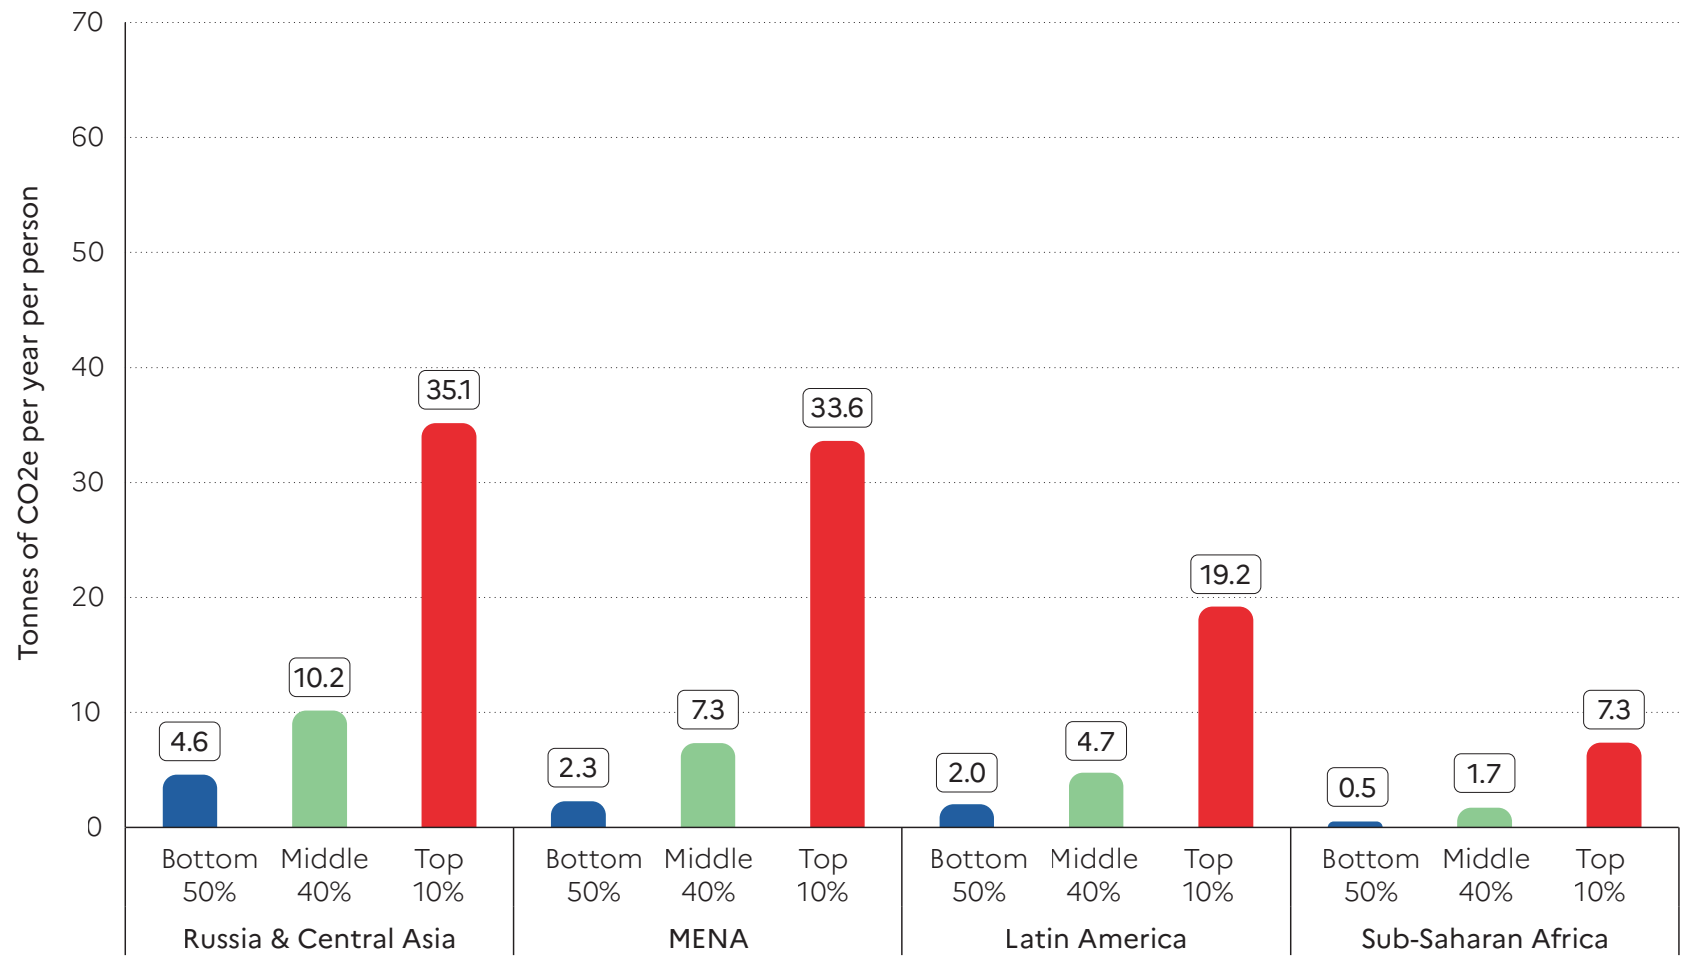
\includegraphics[width=1.0\textwidth]{plots/WIR_carbon_per_capita_rest.png}
      \end{center}      
    \end{columns}

  \end{scriptsize}
  \end{frame}

%%%%%%%%%%%%%%%%%%%%%%%%%%%%%%%%%%%%%%%%%%%%%%%%%%%%%%%%%%%%%%%%%%%%%%%%%%
%%%%%%%%%%%%%%%%%%%%%%%%%%%%%%%%%%%%%%%%%%%%%%%%%%%%%%%%%%%%%%%%%%%%%%%%%%


%%%%%%%%%%%%%%%%%%%%%%%%%%%%%%%%%%%%%%%%%%%%%%%%%%%%%%%%%%%%%%%%%%%%%%%%%%
%%%%%%%%%%%%%%%%%%%%%%%%%%%%%%%%%%%%%%%%%%%%%%%%%%%%%%%%%%%%%%%%%%%%%%%%%%
\begin{frame}
  \begin{small}
              
  \begin{columns}
  \column{0.9\textwidth}
  {\cb Intergovernmental Panel on Climate Change (IPCC) Assessment Report 6 (2021)}
    \begin{itemize}\setlength\itemsep{1.0ex}\footnotesize
      \item[1.]  \hhref{https://report.ipcc.ch/ar6wg2/pdf/IPCC_AR6_WGII_SummaryForPolicymakers.pdf}{Working Group II: Impacts, Adaptation and Vulnerability}
    \end{itemize}
  \end{columns}

  \end{small}
\end{frame}  

%%%%%%%%%%%%%%%%%%%%%%%%%%%%%%%%%%%%%%%%%%%%%%%%%%%%%%%%%%%%%%%%%%%%%%%%%%%%%%%%%%
\begin{frame}
  \frametitle{\centerline{\hhref{https://report.ipcc.ch/ar6wg2/pdf/IPCC_AR6_WGII_SummaryForPolicymakers.pdf}{IPCC Impacts, Adaptation and Vulnerability:} Climate change impact on natural ecosystems}}
  \begin{scriptsize}

    \begin{columns}
      \column{1.0\textwidth}
      \begin{itemize}\setlength\itemsep{1.9ex}        
        \item[o] A
      \end{itemize}

    \end{columns}

    \vspace{-0.1cm}
    \begin{columns}
      \column{0.9\textwidth}
      \begin{center}
          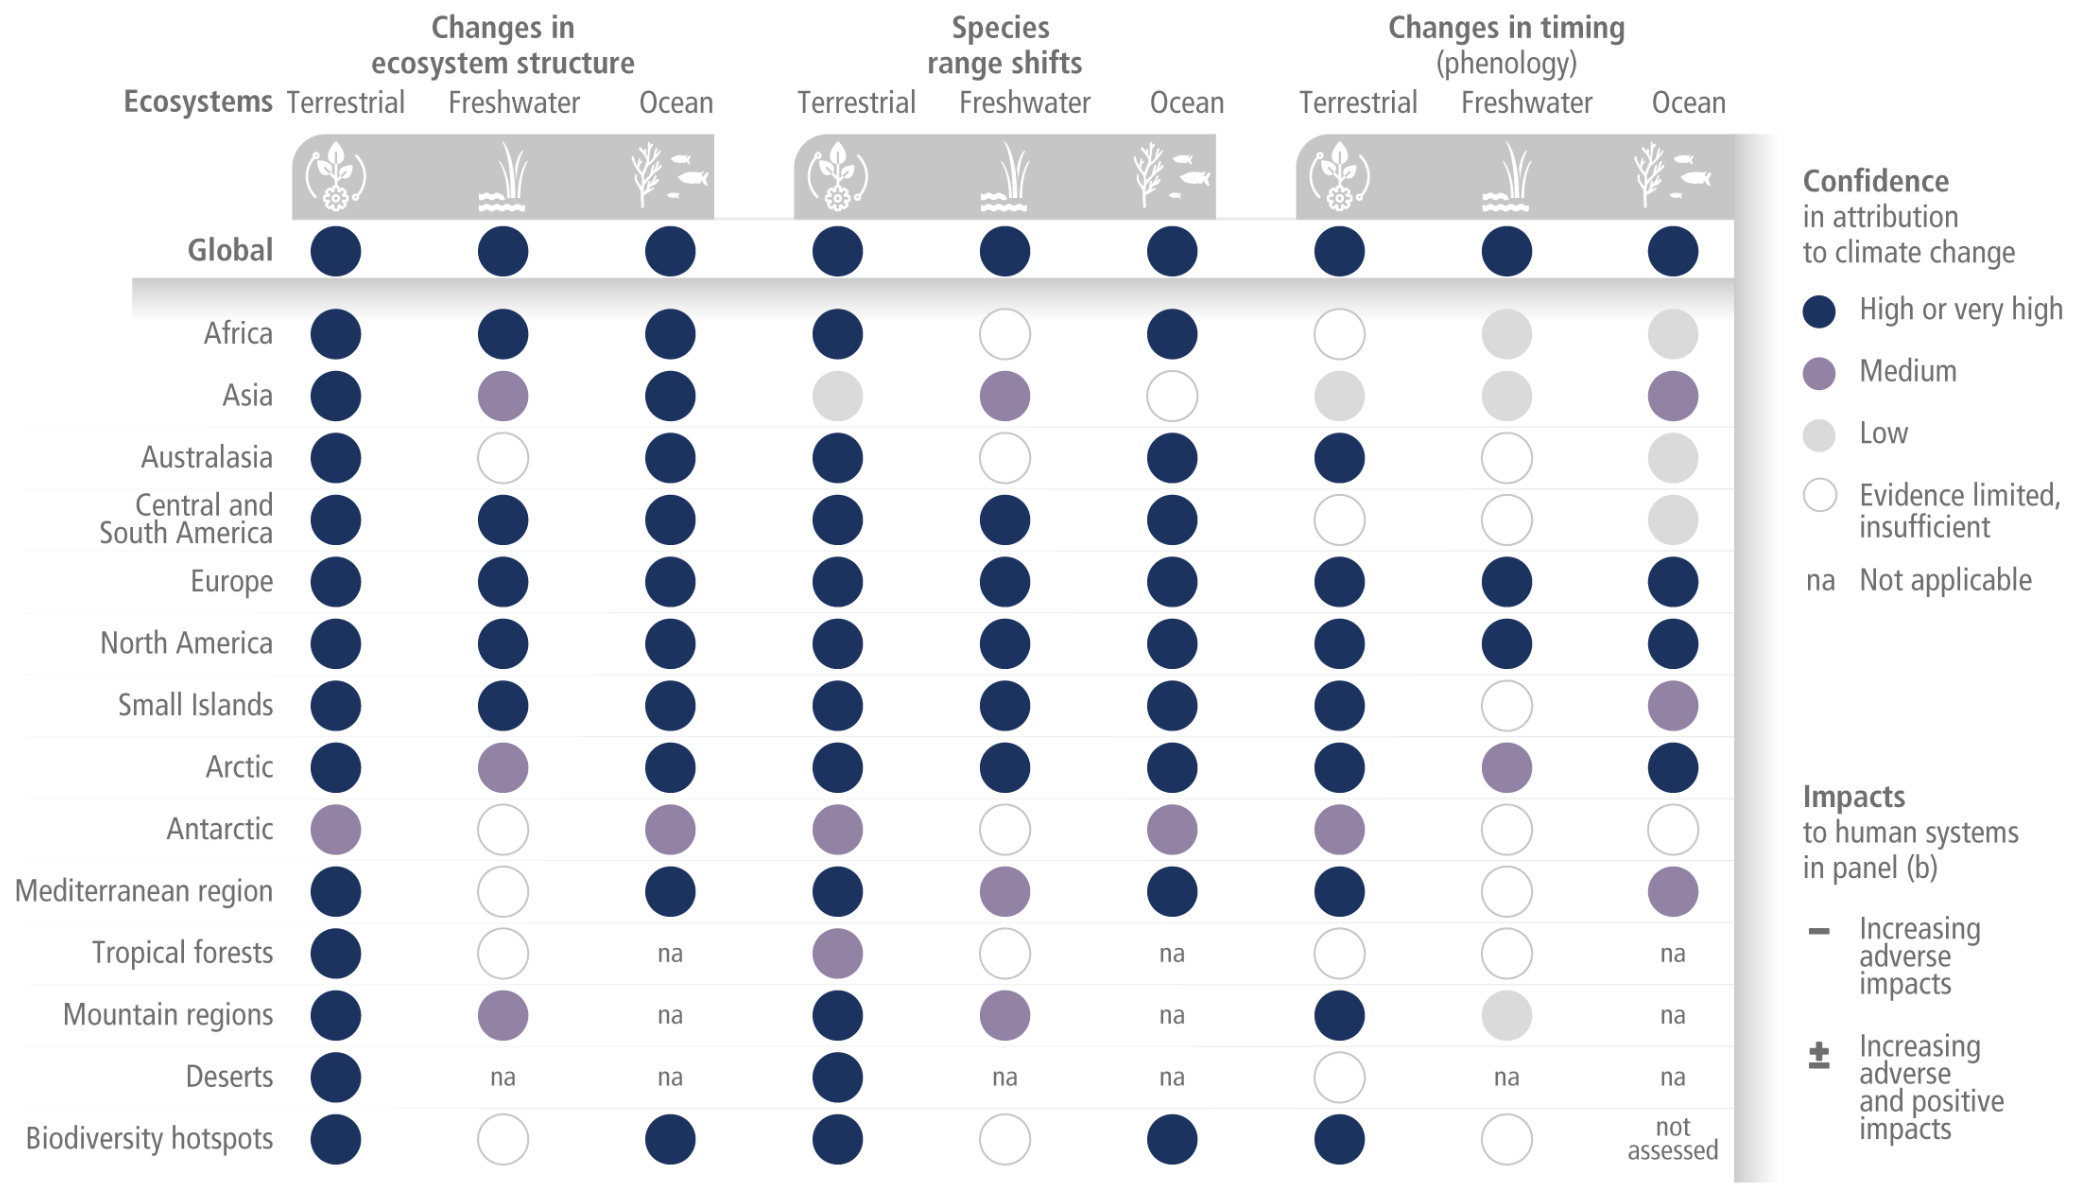
\includegraphics[width=1.0\textwidth]{plots/WG2_impact_on_ecosystems.png}
      \end{center}   
    \end{columns}

  \end{scriptsize}
  \end{frame}  

%%%%%%%%%%%%%%%%%%%%%%%%%%%%%%%%%%%%%%%%%%%%%%%%%%%%%%%%%%%%%%%%%%%%%%%%%%%%%%%%%%
\begin{frame}
  \frametitle{\centerline{\hhref{https://report.ipcc.ch/ar6wg2/pdf/IPCC_AR6_WGII_SummaryForPolicymakers.pdf}{IPCC Impacts, Adaptation and Vulnerability:} Climate change impact on human societies}}
  \begin{scriptsize}

    \begin{columns}
      \column{1.0\textwidth}
      \begin{itemize}\setlength\itemsep{1.9ex}        
        \item[o] B
      \end{itemize}

    \end{columns}

    \vspace{-0.1cm}
    \begin{columns}
      \column{0.9\textwidth}
      \begin{center}
          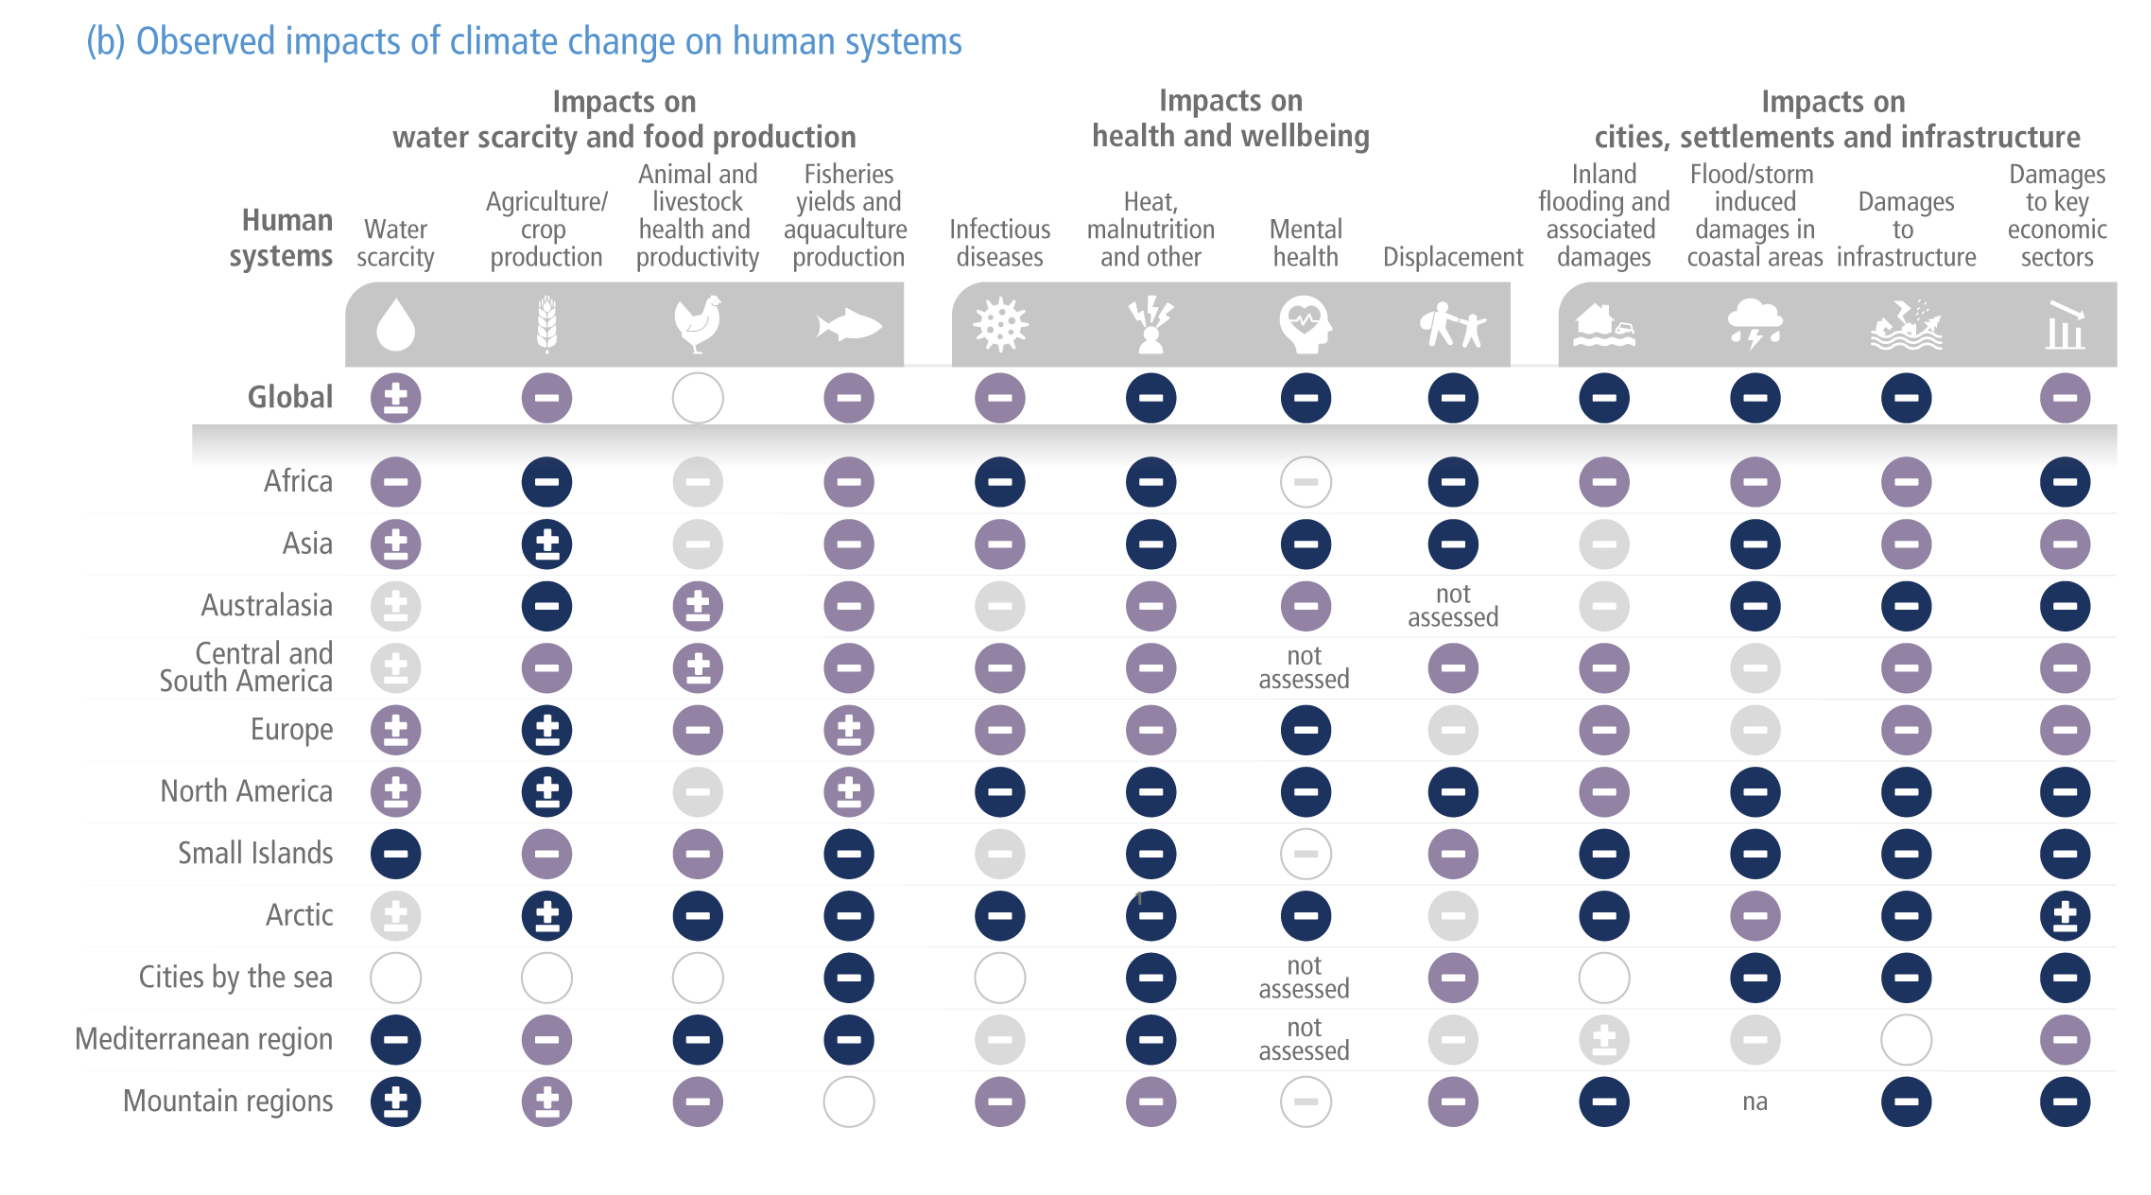
\includegraphics[width=1.0\textwidth]{plots/WG2_impact_on_society.png}
      \end{center}   
    \end{columns}

  \end{scriptsize}
  \end{frame}  

%%%%%%%%%%%%%%%%%%%%%%%%%%%%%%%%%%%%%%%%%%%%%%%%%%%%%%%%%%%%%%%%%%%%%%%%%%
%%%%%%%%%%%%%%%%%%%%%%%%%%%%%%%%%%%%%%%%%%%%%%%%%%%%%%%%%%%%%%%%%%%%%%%%%%


%%%%%%%%%%%%%%%%%%%%%%%%%%%%%%%%%%%%%%%%%%%%%%%%%%%%%%%%%%%%%%%%%%%%%%%%%%
%%%%%%%%%%%%%%%%%%%%%%%%%%%%%%%%%%%%%%%%%%%%%%%%%%%%%%%%%%%%%%%%%%%%%%%%%%
\begin{frame}
  \begin{small}
              
  \begin{columns}
  \column{0.9\textwidth}
  {\cb Intergovernmental Panel on Climate Change (IPCC) Assessment Report 6 (2021)}
    \begin{itemize}\setlength\itemsep{1.0ex}\footnotesize
      \item[1.]  \hhref{https://www.ipcc.ch/report/ar6/wg3/downloads/report/IPCC_AR6_WGIII_SPM.pdf}{Working Group III:  Mitigation of Climate Change}
    \end{itemize}
  \end{columns}

  \end{small}
\end{frame}  

%%%%%%%%%%%%%%%%%%%%%%%%%%%%%%%%%%%%%%%%%%%%%%%%%%%%%%%%%%%%%%%%%%%%%%%%%%%%%%%%%%
\begin{frame}
  \begin{scriptsize}

    \vspace{-0.1cm}
    \begin{columns}
      \column{0.43\textwidth}
      \begin{center}
          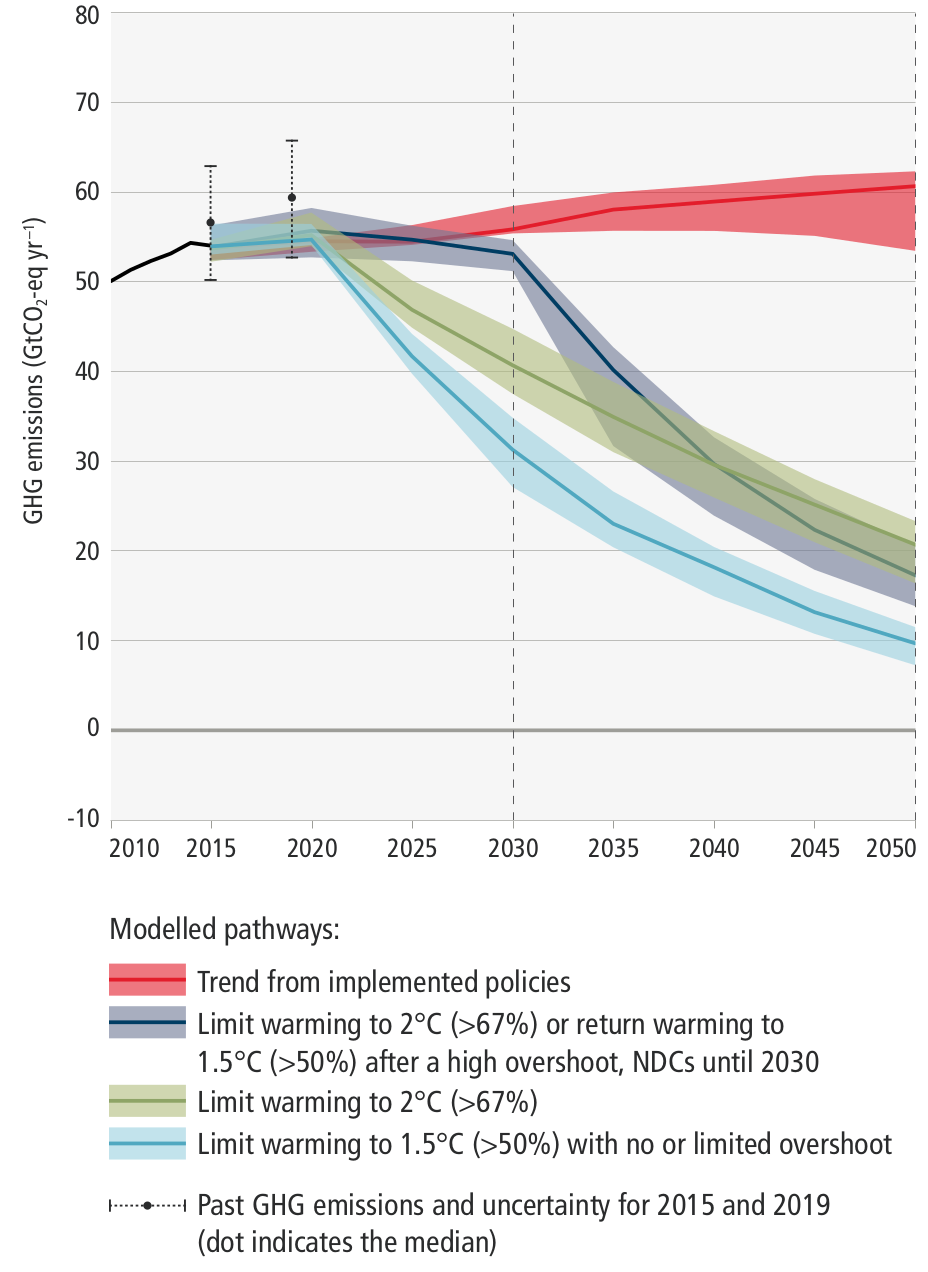
\includegraphics[width=1.0\textwidth]{plots/WG3_global_GHG_emissions.png}
      \end{center}  
      
      \column{0.5\textwidth}
      \begin{itemize}\setlength\itemsep{1.9ex}        
        \item[o] \hhref{https://www.ipcc.ch/report/ar6/wg3/downloads/report/IPCC_AR6_WGIII_SPM.pdf}{IPCC  Mitigation of Climate Change:}
      \end{itemize}

    \end{columns}

  \end{scriptsize}
  \end{frame}  

%%%%%%%%%%%%%%%%%%%%%%%%%%%%%%%%%%%%%%%%%%%%%%%%%%%%%%%%%%%%%%%%%%%%%%%%%%%%%%%%%%
\begin{frame}
  \frametitle{\centerline{\hhref{https://www.ipcc.ch/report/ar6/wg3/downloads/report/IPCC_AR6_WGIII_SPM.pdf}{IPCC  Mitigation of Climate Change:} Climate change impact on natural ecosystems}}
  \begin{scriptsize}

    \begin{columns}
      \column{1.0\textwidth}
      \begin{itemize}\setlength\itemsep{1.9ex}        
        \item[o] A
      \end{itemize}

    \end{columns}

    \vspace{-0.1cm}
    \begin{columns}
      \column{0.99\textwidth}
      \begin{center}
          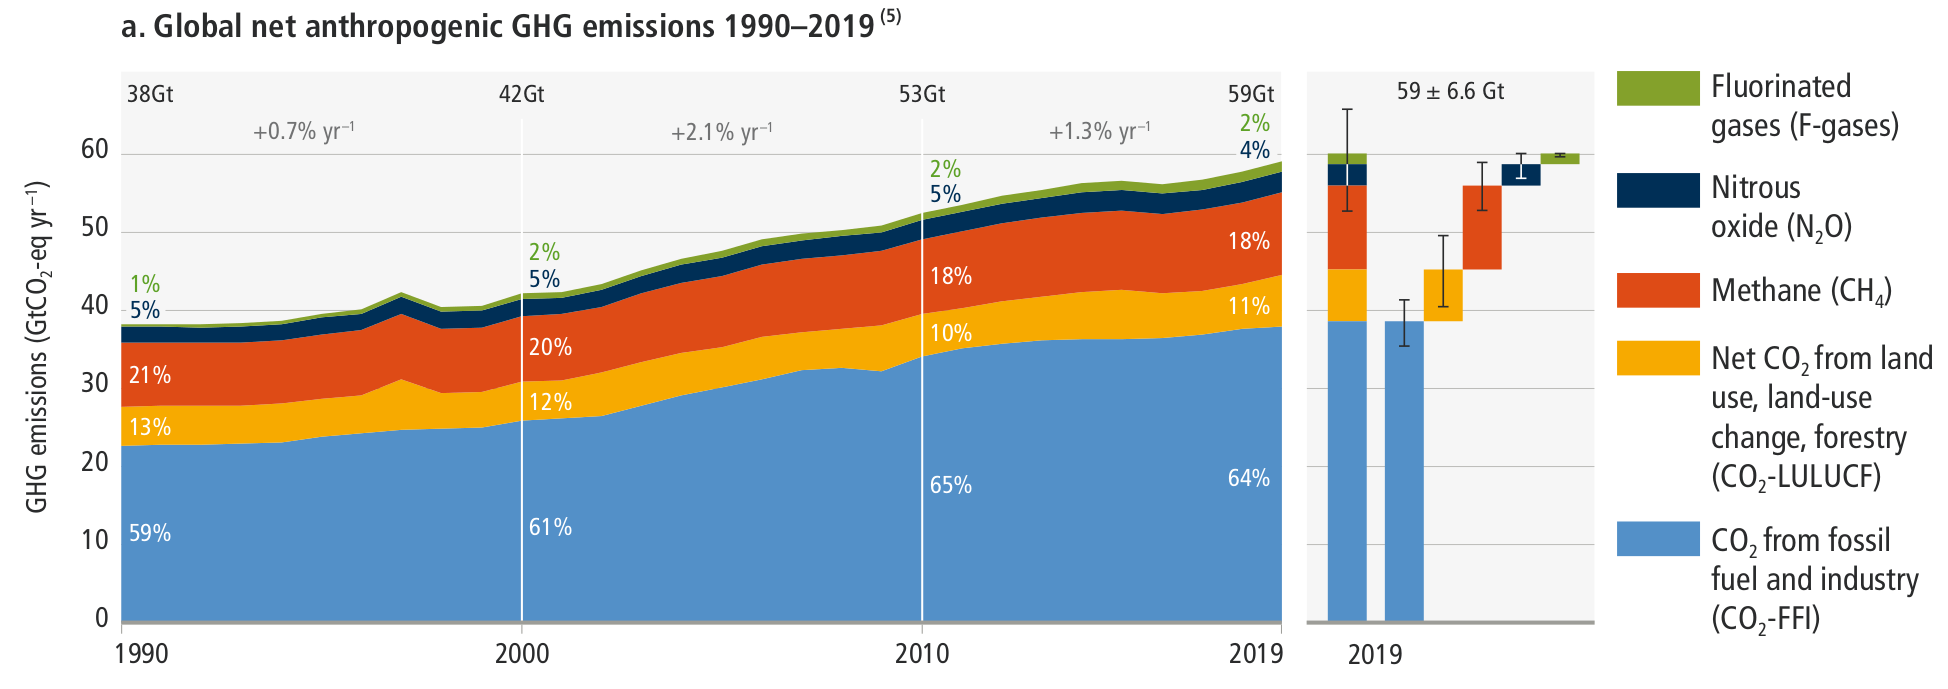
\includegraphics[width=1.0\textwidth]{plots/WG3_net_greenhouse_emissions.png}
      \end{center}   
    \end{columns}

  \end{scriptsize}
  \end{frame} 

  
%%%%%%%%%%%%%%%%%%%%%%%%%%%%%%%%%%%%%%%%%%%%%%%%%%%%%%%%%%%%%%%%%%%%%%%%%%%%%%%%%%
\begin{frame}
  \begin{scriptsize}

    \vspace{-0.1cm}
    \begin{columns}
      \column{0.52\textwidth}
      \begin{center}
          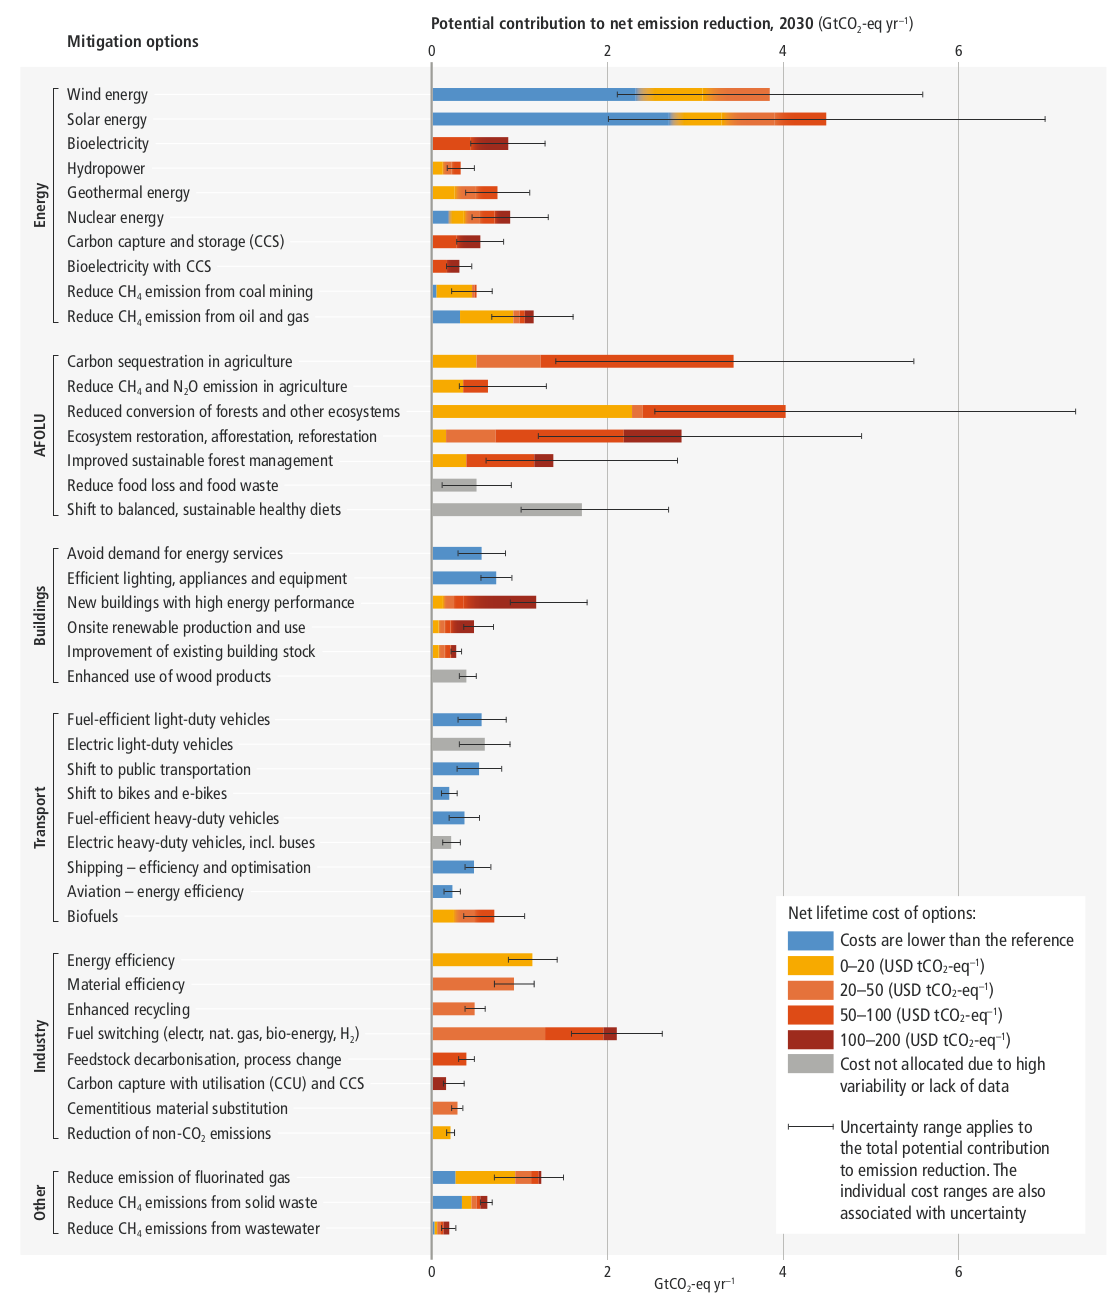
\includegraphics[width=1.0\textwidth]{plots/WG3_mitigation_options.png}
      \end{center}   

      \column{0.4\textwidth}
      \begin{itemize}\setlength\itemsep{1.9ex}        
        \item[o] \hhref{https://www.ipcc.ch/report/ar6/wg3/downloads/report/IPCC_AR6_WGIII_SPM.pdf}{IPCC  Mitigation of Climate Change}
      \end{itemize}
    \end{columns}

  \end{scriptsize}
  \end{frame} 

%%%%%%%%%%%%%%%%%%%%%%%%%%%%%%%%%%%%%%%%%%%%%%%%%%%%%%%%%%%%%%%%%%%%%%%%%%%%%%%%%%
\begin{frame}
  \begin{scriptsize}
              
  \vspace{-0.1cm}
  \begin{columns}
    \column{0.25\textwidth}
   Sources of CO$_2$ emissions in France:\\
   \vspace{0.1cm} 
   \hhref{https://rustem.web.cern.ch/climate/LeMondeClimateEmergencyFranceImpact.pdf}{Le Monde, May 30th, 2022}

    \column{0.55\textwidth}
    \begin{center}
        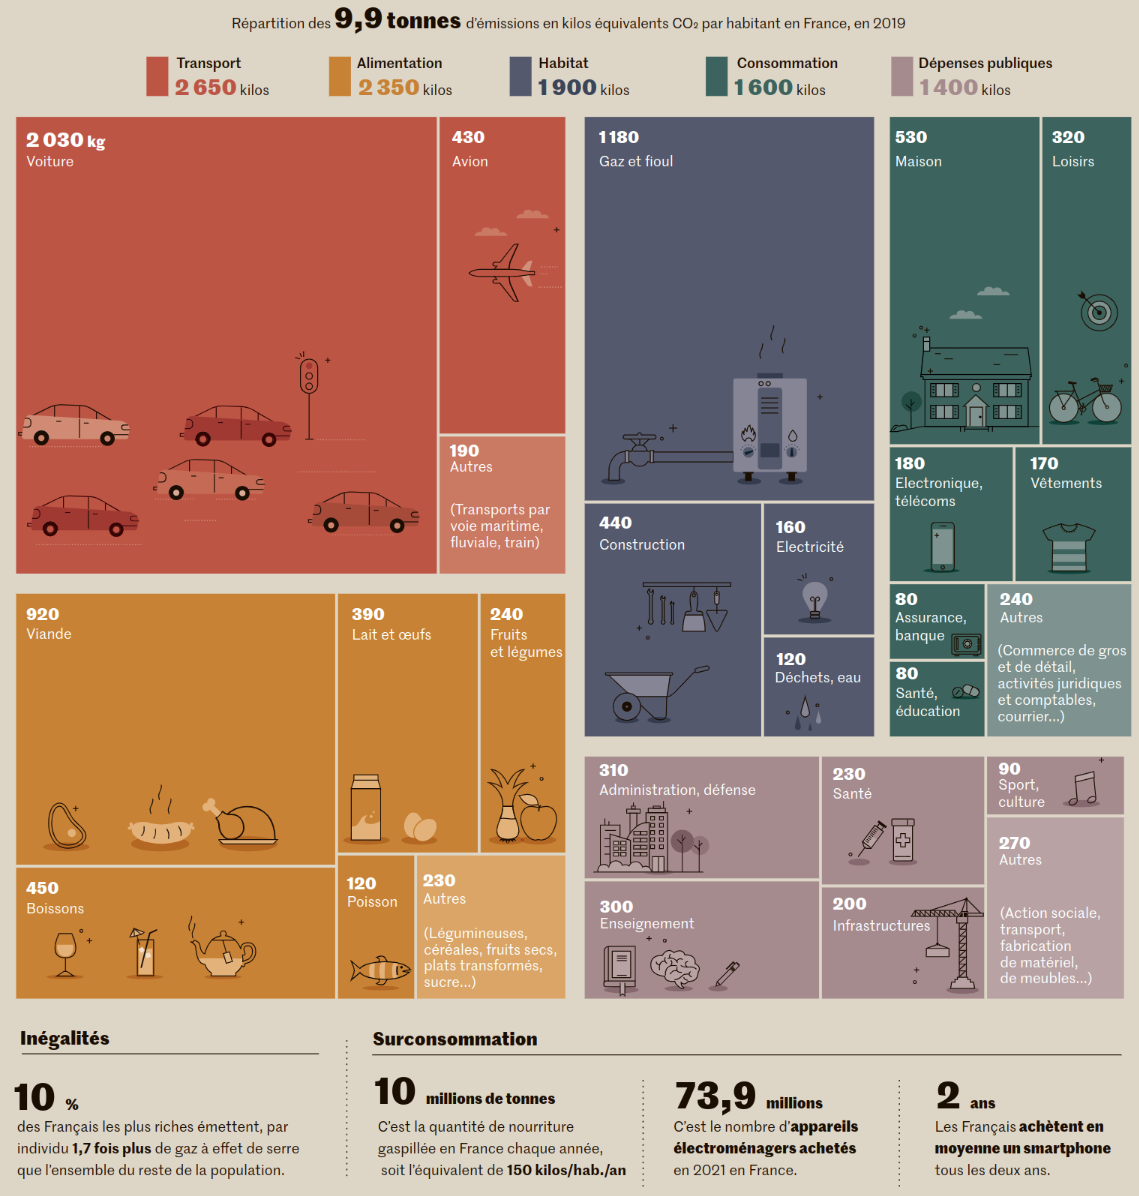
\includegraphics[width=1.0\textwidth]{plots/co2_breakdown.png}
    \end{center}
  \end{columns}

  \end{scriptsize}
  \end{frame}

  %%%%%%%%%%%%%%%%%%%%%%%%%%%%%%%%%%%%%%%%%%%%%%%%%%%%%%%%%%%%%%%%%%%%%%%%%%%%%%%%%%
  \begin{frame}
    \frametitle{\centerline{Summary}}
    \begin{footnotesize}
  
      \begin{columns}
        \column{1.0\textwidth}
        \begin{itemize}\setlength\itemsep{2.9ex}        
          \item[o] Global surface temperature will continue to increase until at least mid-century under all considered emissions scenarios.
  
          \item[o] Global warming of 1.5$^\circ$C and 2$^\circ$C will be exceeded during the 21st century, unless deep reductions in CO$_2$ and other greenhouse gas emissions occur in the coming decades.
  
          \item[o]  Extreme weather, rising seas and damaged ecosystems could threaten the safety and livelihoods of billions of people in the next decades. 

          \item[o] {\bf There could be 1.2 billion climate refugees by 2050} - \hhref{https://www.zurich.com/en/media/magazine/2022/there-could-be-1-2-billion-climate-refugees-by-2050-here-s-what-you-need-to-know}{Ecological Threat Register}
      \end{itemize}
      \end{columns}

  
    \end{footnotesize}
    \end{frame}  

%%%%%%%%%%%%%%%%%%%%%%%%%%%%%%%%%%%%%%%%%%%%%%%%%%%%%%%%%%%%%%%%%%%%%%%%%%%%%%%%%%
\end{document}